\documentclass[12pt,a4paper, spanish]{report}
\usepackage[spanish]{babel}
\usepackage[latin1]{inputenc}  % Ambos para solucin de asuntos de idioma
\usepackage[T1]{fontenc}
\usepackage{tocbibind}  % Bibliografa en el indice
\usepackage{titlesec}  % Posibilidad de editar los formatos de chapter y section
%\usepackage{times}  % Fuente de letras
\usepackage{amsmath,amssymb,mathrsfs,mathptmx}  % Matemticas varias
\usepackage{hyperref} % Para escribir URLs



% --- Arreglos varios para la inclusion de imgenes
%\usepackage[pdftex]{graphicx}
%\usepackage[dvips]{graphicx}
\usepackage{graphicx}
\usepackage{epstopdf}
\usepackage{float}
\usepackage{subfigure}
%\usepackage{subfig}
\usepackage{wrapfig}
\usepackage[usenames,dvipsnames]{color}
\DeclareGraphicsExtensions{.png,.jpg,.pdf,.mps,.gif,.bmp, .eps}


	

\usepackage{multirow}
\usepackage{multicol}
\usepackage{tabulary}
\usepackage[table]{xcolor}
\usepackage{color}
\usepackage{listings}
%\usepackage{subfloat}
\usepackage{tikz}

\setcounter{secnumdepth}{3}
\setcounter{tocdepth}{3}


% --- Para las dimensiones de los mrgenes etc
\frenchspacing \addtolength{\hoffset}{-1.5cm}
\addtolength{\textwidth}{3cm} \addtolength{\voffset}{-2.5cm}
\addtolength{\textheight}{4cm}
% --- Para el encabezado
\usepackage{fancyhdr}
\fancyhead[R]{2012}\fancyhead[L]{enCuadro} \fancyfoot[C]{\thepage}
\pagestyle{fancy}

% --- Formato de la etiqueta Chapter
%\newcommand{\bigrule}{\titlerule[0.5mm]}
%\titleformat{\chapter}[display]{\bfseries\Huge}
%{\Large\chaptertitlename\ \Large\thechapter}
%{0mm} {\filleft} [\vspace{0.5mm} \bigrule]

\titleformat{\chapter}[display]
{\normalfont\Large\filcenter}
{\titlerule[1pt]%
\vspace{1pt}%
\titlerule
\vspace{1pc}%
\LARGE\MakeUppercase{\chaptertitlename} \thechapter}
{1pc}
{\titlerule
\vspace{1pc}%
\Huge}

%-------------------------

\begin{document}
% Esto es para que se muestren todas las referencias aunque no se citen:
\nocite{*}

\renewcommand{\tablename}{Tabla}
\renewcommand{\theenumi}{\Roman{enumi}}
\renewcommand{\labelenumi}{[\textbf{\theenumi}]}
\renewcommand{\thefootnote}{\arabic{footnote}}
% --- Modificacin de entornos enumerate
\renewcommand{\theenumi}{\roman{enumi}}
\renewcommand{\labelenumi}{\theenumi)}
% --- Modificacin de entornos enumerate

% --- Para hacer highlights
\newcommand{\highlAmarillo}[1]{\colorbox{yellow}{#1}}
\newcommand{\highlVerde}[1]{\colorbox{green}{#1}}
\newcommand{\highlRojo}[1]{\colorbox{red}{#1}}

%



\chapter{Hardware y Software}
\label{chap: hwysw}
\section{Introducci�n}
Introducci�n
\section{Software de procesamiento de im�genes}
Software de procesamiento de im�genes
\subsection{Lenguaje C}
Ventajas del Lenguaje C para procesamiento de im�genes
\subsection{Librer�as y recursos}
\subsubsection{OpenCV}
\subsubsection{IPOL}
\subsubsection{ITK e ImageMagik}

\section{Elecci�n de plataforma}
La elecci�n de la plataforma para desarrollar fue una de las primeras desiciones que se tuvo que hacer m�s all� del proceso natural inicial de investigaci�n del proyecto. Esto es debido a que existen muchos factores que se ven afectados en funci�n de la plataforma que se eligiera que van desde aprendizaje de lenguaje, entorno de desarrollo hasta la adquisici�n de plataformas y/o m�quinas para desarrollar. As� entonces las dos grandes posibilidades que se ten�an al comienzo y que determinaban estos factores era la elecci�n de trabajar en plataformas que tuvieran los sistemas operativos Android o iOS (en ning�n momento se consider� desarrollar sobre plataformas con Symbian dado que est� en proceso de desaparici�n). Uno de los aspectos desfavorables que se ve�a sobre Android era la multiplicidad de plataformas existentes, de distintas caracter�sticas de procesamiento, c�mara y sensores entre otras cosas con respecto a las plataformas que utilizan iOS. Por otra parte luego de un proceso de investigaci�n se vio que el conjunto de herramientas existentes y el estado de maduraci�n del desarrollo de aplicaciones para iOS hac�an de este sistema operativo, un camino m�s seguro para comenzar en un �rea que era desconocida. Es sabido que Android es un sistema operativo que viene en pleno crecimiento y que a nivel masivo es una buena alternativa desarrollar en �l, pero para los fines de investigaci�n y de desarrollo de sotware que ten�a el presente proyecto se vio que era mejor desarrollar sobre iOS y plataformas Apple.\\

Al trabajar con Apple entonces se cuenta con la ventaja de contar con pocas variantes en cuanto al Hardware utilizado. B�sicamente existen tres familias de dispositivos en los que se puede desarrollar: iPhone, iPad y iPod Touch. Para cada variante de plataforma existen distintos modelos que hacen que algunas caracter�sticas importantes como la capacidad de procesamiento, la resoluci�n de c�mara o el tama\~no de la pantalla entre otras puedan verse afectadas. A continuaci�n se presenta brevemente c�mo fue el surgimiento de cada uno de los dispositivos al mercado y se describen resumidamente las principales caracter�sticas.
\subsection{iPhone, iPad, iPod Touch}
\subsubsection{Comparaci�n de plataformas.}
Sin dudas el iPhone fue uno de los saltos m�s grandes en el mundo tecnol�gico en los �ltimos a\~nos. Logr� llenar el hueco que los PDAs de la d�cada de los 90 no hab�an sabido completar y comenz� a desplazar al invento que revolucion� el mercado de los contenidos de m�sica, el iPod. Gracias a su pantalla t�ctil capacitiva de alta sensibilidad logr� reunir todas las funcionalidades agregando solamente un gran bot�n y algunos extra para controlar volumen o desbloquar el dispositivo. \\
La primera generaci�n del iPhone fue lanzada por Apple en Junio de 2007 en Estados Unidos, luego de una gran inversi�n de la operadora AT\&T que exig�a exclusividad de venta dentro de dicho pa�s durante los siguientes cuatro a\~nos. La misma soportaba tecnolog�a GSM cuatribanda y se lanz� en dos variantes de 4GB y 8GB de ROM. El segundo modelo lanz� como novedad el soporte de tecnolog�a 3G cuatribanda y GPS asistido. Luego le siguieron el iPhone 3GS, 4, 4S y el 5, siendo este �ltimo, la sexta y �ltima generaci�n disponible al momento de la redacci�n de este trabajo.\\

%http://ipod.about.com/od/ipadcomparisons/a/ipad-iphone-3gs-ipod-touch.htm
%http://www.apple.com/ipod-touch/specs.html
%http://www.apple.com/iphone/specs.html
%http://www.apple.com/ipod-touch/fourth-generation-specs.html
%http://www.apple.com/ipad/compare/

%http://en.wikipedia.org/wiki/List_of_iOS_devices
%http://en.wikipedia.org/wiki/IPod_Touch
%http://en.wikipedia.org/wiki/IPhone
%http://en.wikipedia.org/wiki/IPad

%SUPPORT
%http://support.apple.com/kb/SP587
%http://support.apple.com/kb/SP643
%http://support.apple.com/kb/SP594
%http://support.apple.com/kb/SP622

%PLATFORM NOTES
%http://developer.apple.com/library/ios/#documentation/3DDrawing/Conceptual/OpenGLES_ProgrammingGuide/OpenGLESPlatforms/OpenGLESPlatforms.html

%BENCHMARK GPU
%http://www.anandtech.com/show/4216/apple-ipad-2-gpu-performance-explored-powervr-sgx543mp2-benchmarked

%COMPARE
%http://www.gsmarena.com/compare.php3

%GPU SGX
%http://developer.apple.com/library/ios/#documentation/3DDrawing/Conceptual/OpenGLES_ProgrammingGuide/OpenGLESPlatforms/OpenGLESPlatforms.html
Por su parte tanto el iPad como el iPod Touch tambi�n representaron un gran salto en el mundo de las plataformas y \textit{Tablets}, agrandando las posibilidades de desarrollo y procesamiento. Como se dijo, de cada una de estas tres familias de dispositivos existen distintas versiones y modelos. Por eso, a continuaci�n se muestra una tabla comparativa de determinadas caracter�sticas que son de inter�s a los 
efectos del presente proyecto.

\tiny
\begin{table}[htbp]
\caption{Comparativa de algunas plataformas Apple}
\begin{tabular}{|l|l|l|l|l|}
\hline
& \textbf{iPhone 4} & \textbf{iPhone 4s} & \textbf{iPod Touch 4G} & \textbf{iPad 2} \\ \hline

\textbf{ROM} & \scriptsize 8, 16 o 32 GB & \scriptsize 16, 32 o 64 GB & \scriptsize 8, 32 o 64 GB & \scriptsize  16, 32 o 64 GB \\ \hline

\textbf{RAM} & \scriptsize 512 MB  & \scriptsize 512 MB & \scriptsize 256 MB & \scriptsize 512 MB \\ \hline

\textbf{SoC} & \scriptsize Apple A4 & \scriptsize Apple A5 & \scriptsize Apple A4 & \scriptsize Apple A5 \\ \hline

\textbf{CPU} & \scriptsize 1 GHz, ARM Cortex-A8 & \scriptsize 1 GHz,  dual-core ARM Cortex-A9 & \scriptsize 800 MHz, ARM Cortex-A8 & \scriptsize 1 GHz  dual-core ARM Cortex-A9   \\ \hline

\textbf{GPU} & \scriptsize PowerVR SGX535 GPU & \scriptsize PowerVR SGX543MP2 & \scriptsize PowerVR SGX535 GPU & \scriptsize PowerVR SGX543MP2 \\ 
		    & \scriptsize  & \scriptsize  (2-core) GPU & \scriptsize  & \scriptsize  (2-core) GPU \\ \hline

\textbf{C�MARA} & \scriptsize Foto: 5.0 MP & \scriptsize Foto: 8.0 MP & \scriptsize Foto: 0.7 MP & \scriptsize Foto: 0.7 MP \\ 
				    	& \scriptsize  Video: 720p HD (30 fps) & \scriptsize  Video: 1080p HD (30 fps) & \scriptsize Video: 720p HD (30 fps) & \scriptsize Video: 720p HD (30 fps) \\ \hline

\textbf{PANTALLA} & \scriptsize Diagonal: 3.5'' & \scriptsize Diagonal: 3.5'' & \scriptsize Diagonal: 3.5'' & \scriptsize Diagonal: 9.7'' \\ 
				  & \scriptsize Pixels: 960x640 & \scriptsize Pixels: 960x640 & \scriptsize Pixels: 960x640 & \scriptsize Pixels: 1024x768 \\ 
				  & \scriptsize Densidad de Pixels: 326 ppi  & \scriptsize  Densidad de Pixels: 326 ppi  & \scriptsize Densidad de Pixels: 326 ppi  & \scriptsize  Densidad de Pixels: 123 ppi \\ 
				  & \scriptsize Multit�ctil & \scriptsize Multit�ctil & \scriptsize Multit�ctil & \scriptsize Multit�ctil \\ \hline


\textbf{SENSORES} & \scriptsize Girs�scopo de 3 ejes & \scriptsize Girs�scopo de 3 ejes & \scriptsize Girs�scopo de 3 ejes & \scriptsize Girs�scopo de 3 ejes \\
& \scriptsize Aceler�metro  & \scriptsize Aceler�metro & \scriptsize Aceler�metro & \scriptsize Aceler�metro\\
& \scriptsize Sensor de luz ambiente & \scriptsize Sensor de luz ambiente & \scriptsize  Sensor de luz ambiente & \scriptsize  Sensor de luz \\ 
& \scriptsize Sensor de proximidad & \scriptsize Sensor de proximidad &  & \\ \hline
\end{tabular}
\label{tab: compHWiOS}
\end{table}
\normalsize
%http://www.edaboard.com/thread75452.html

%Microcontroller and System-on-a-chip
%Seminar on Embedded Systems Architecture
%Peter Thoman (peter.thoman@uibk.ac.at)
%University of Innsbruck 2009-12-03
\subsubsection{Algunas caracter�sticas a detallar.}
Hay algunos comentarios respecto de la Tabla \ref{tab: compHWiOS} que es bueno destacar. Primeramente, es importante decir que se eligieron esos cuatro dispositivos pues pareci� de inter�s conocer al menos una plataforma de cada familia y dentro de las mismas se eligieron las que fueron utilizadas para desarrollar.\\
Uno de los puntos a evaluar es el \textbf{SoC}, que refiere a \textit{System on Chip} por sus siglas en ingl�s. \textit{System on Chip} es un concepto de los sistemas embebidos que refiere a la integraci�n de todo lo necesario para poder correr un sistema operativo, en un solo circuito integrado. En contraposici�n a un microcontrolador que es capaz de realizar procesamiento m�s b�sico y menos potente, con poca interacci�n de usuario y menor flexibilidad, un \textit{SoC} refiere a la idea de tener todo lo necesesario para desarrollar sobre la plataforma y poder hacer procesamiento sin tantas limitaciones. B�sicamente cumplen funciones similares pero el \textit{SoC} forma parte de una evoluci�n de los microcontroladores, siendo de una complejidad mayor e integrado en un tama\~no muy reducido buscando poco consumo y eficiencia de costos. As� entonces un \textit{SoC} puede estar conformado por un microcontrolador y hardware adicional como procesadores de se\~nal y bloques de memoria.  \\
%http://www.arm.com/products/processors/cortex-a/index.php
En la Figura \ref{fig: soc} se ilustran los dos tipos de \textit{SoC} de los dispositivos de la Tabla \ref{tab: compHWiOS}: Apple A4 y Apple A5. Algunos dispositivos que no figuran en la tabla como el \textit{iPhone 5} o el \textit{iPad 4} usan \textit{SoCs} m�s recientes como el Apple A6 o Apple A6x respectivamente. La familia de \textit{SoCs} Apple Ax, es la que la mencionada firma utiliza en todas sus plataformas, inclusive en el \textit{Apple TV} y es manufacturada por Samsung. Estos \textit{SoCs} se caracterizan por utilizar CPUs de arquitectura ARM, en su mayor�a ARMv7 y GPUs de PowerVR de la l�nea SGX. \\

\begin{figure}[h!]
\centering
$
\begin{array}{cc}
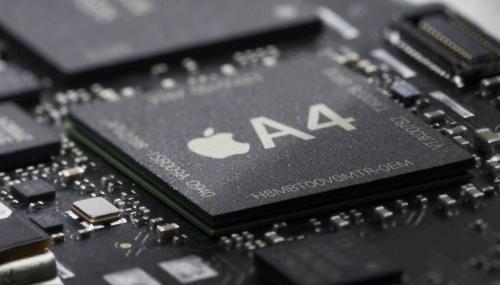
\includegraphics[scale=0.3]{figs_hwysw/applea4.png} & 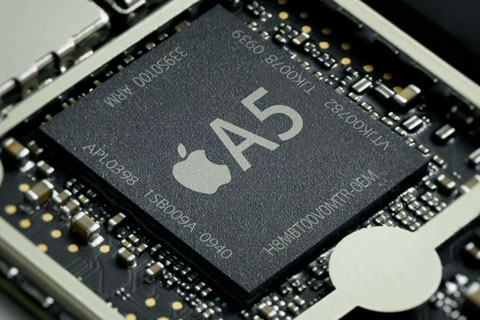
\includegraphics[scale=0.3]{figs_hwysw/applea5.png} \\
\end{array}
$
\caption{\textit{System on Chip}: SoC.}
\label{fig: soc}
\end{figure}

La arquitectura ARM incorpora algunas caracter�sticas de la arquitectura RISC (\textit{Reduced Instruction Set Computer}) como el hecho que las operaciones sean llevadas a cabo sobre un conjunto de registros a tales efectos y no sobre la memoria directamente. Otra caracter�stica que tiene de RISC es que tiene un modo simple de direccionamiento donde las direcciones son tambi�n guardadas sobre registros destinados a tales efectos. La mayor�a de los procesadores est�n hechos con un ancho de palabra de 32-bit salvo el reciente ARMv8 que incorpora la posibilidad de utilizar ambos anchos de palabra: 32-bit o 64-bit. Otra caracter�stica a destacar sobre estos procesadores es que es posible programar sobre ellos utilizando lenguaje C/C++. Por m�s informaci�n sobre esta arquitectura referirse a la web de la empresa \url{http://www.arm.com}.\\
Por su parte las GPU utilizadas en los \textit{SoCs} de la serie Apple Ax, son GPUs de PowerVR, una divisi�n de la firma Imagination Technologies (\url{http://www.imgtec.com/}) que desarrolla hardware y software para \textit{rendering} 2D y 3D, procesamiento de im�genes y codificaci�n. La funci�n que tiene la GPU es asignar a cada pixel de la pantalla su color para cada cuadro. En particular, estas GPU implementan un concepto innovador de \textit{renderizado} que mejora notoriamente la performance de los gr�ficos: \textit{Tile-Bassed Deferred Rendering} (TBDR). Este concepto aprovecha la independencia de �reas alejadas de la pantalla y de la correlaci�n de p�xeles cercanos y divide la pantalla en \textit{tiles} o baldozas. A cada \textit{tile} se le asocia un procesamiento paralelo y con esto se mejora notablemente la performance respecto al m�todo tradicional: Immediate mode renderers (IMRs), que procesa la pantalla completa. Las im�genes \textit{renderizadas} est�n hechas por tri�ngulos (pol�gonos), por lo que uno de los indicadores fundamentales para evaluar la performance de una GPU es la cantidad de tri�ngulos (pol�gonos) que es capaz de procesar por segundo. En (referencia benchmark: http://www.anandtech.com/show/4216/apple-ipad-2-gpu-performance-explored-powervr-sgx543mp2-benchmarked) se puede ver un an�lsis interesante que compara entre otros, a los dos tipos de GPU que se presentaron en la Tabla \ref{tab: compHWiOS}: SGX535 y SGX543MP2. En dicho an�lisis se muestra por ejemplo que en el mejor de los casos la GPU SGX535 fue capaz de procesar 8.69 millones de tri�ngulos por segundo frente a los 29 millones procesados por la GPU SGX543MP2.\\
%http://www.imgtec.com/powervr/powervr-graphics-technology.asp


\section{Software de Apple Inc.}

\subsection{Sistemas Operativos}
Para poder desarrollar aplicaciones sobre dispositivos m�viles de la firma Apple Inc. es necesario contar con computadoras que corran el sistema operativo \textbf{Mac OS X}. Esto puede ser llevado a cabo, ya sea adquiriendo plataformas de desarrollo de la mencionada firma o creando m�quinas virtuales que corran dicho sistema operativo. Para la segunda opci�n (la m�s econ�mica pero con ciertas dificultades de performance), es necesario que la computadora cuente con virtualizaci�n de hardware. Se comenz� trabajando de esta manera hasta el momento de adquirir plataformas de desarrollo que contaran con Mac OS X en forma nativa.\\
Mac OS X refiere a la versi�n n�mero 10 (en n�meros romanos) de una serie de sistemas operativos que comenzaron a desarrollarse en la d�cada de los 80 (Mac OS 1 data del a?o 1984). En los �ltimos 28 a?os se han ido sucediendo nuevas versiones que han ido mejorando caracter�sticas en la estructura de datos con la incorporaci�n de la jerarqu�a de archivos en Mac OS 3 por ejemplo, en la b�squeda de archivos, con la simultaneidad de tareas, multiplicidad de usuarios o incluso con el �nfasis en la interfaz de usuario por mencionar algunas caracter�sticas importantes en la evoluci�n de esta familia de sistemas operativos. Dentro de Mac OS X existen distintas versiones, siendo la m�s actual la Versi�n 10.8: Mountain Lion lanzada durante 2012.\\
Por su parte todas las plataformas m�viles de Apple Inc corren otro dispositivo de c�digo cerrado: \textbf{iOS}. Originalmente llamado as� por ser el sistema operativo utilizado por la plataforma iPhone, este sistema operativo est� tambi�n en las plataformas iPad, iPod Touch y Apple TV en todas sus versiones. La versi�n m�s reciente de este SO es el iOS 6.1.\\
Una de las grandes innovaciones de estas plataformas es el hecho de poder desarrollar aplicaciones y correrlas en el propio dispositivo (por supuesto tambi�n sucede lo mismo en el mundo Android). Para poder lograr esto, es necesario como se ha dicho, contar con una m�quina que corra Mac OS X y contar con el SDK apropiado llamado \textbf{Xcode}. Este entorno de desarrollo y su lenguaje se explican en la secci�n \ref{sec: objc}.

\subsection{Objective-C}
\label{sec: objc}
%http://developer.apple.com/library/mac/#documentation/Cocoa/Conceptual/ObjectiveC/Introduction/introObjectiveC.html
El lenguaje que fue elegido por Apple Inc para desarrollar sobre plataformas m�viles es Objective-C. Este lenguaje fue desarrollado en la d�cada de 1980 como un superconjunto de C orientado a objetos. Es decir que es una extensi�n del standard ANSI C que incorpora un modelo orientado a objetos basado en \textbf{Smalltalk}. Una de las diferencias sustanciales del modelo orientado a objetos de Objective-C respecto a otros lenguajes como Java o C++, es el hecho de la invocaci�n de los m�todos (procedimientos) de las instancias de clases. En objective-C esta invocaci�n se da enviando mensajes, algo que se hereda de Smalltalk. As� entonces para invocar un m�todo se procede con el siguiente c�digo por ejemplo:
\begin{verbatim}
[receiver message];
\end{verbatim}
Donde $receiver$ es un objeto que recibe un mensaje (acci�n) $message$ a realizar. Esta acci�n puede tener par�metros asociados, como por ejemplo el siguiente c�digo real:
\begin{verbatim}
[myRectangle setWidth:20.0];
\end{verbatim}
Esta diferencia conceptual de utilizar mensajes se representa en el hecho de que en tiempo de compilaci�n estos mensajes no son m�s que una etiqueta y no est�n asociados al bloque de c�digo como es el caso de Java o C++. Entonces es factible que suceda el hecho de que ese mensaje o m�todo no est� implementado por esa clase y reci�n en tiempo de ejecuci�n es que saltar� el error al sustituirse esa etiqueta por un c�digo inexistente, pues un objeto recibe un mensaje para realizar un m�todo que no est� dentro de su repertorio. Para esto es que en la documentaci�n de Apple Inc se recomienda utilizar ciertos trucos para garantizar que el objeto que reciba el mensaje sea capaz de responder correctamente, como por ejemplo consultando primero si es capaz de realizar dicha acci�n y luego en caso de poder realizar dicha acci�n.\\
Otro detalle a destacar es que este lenguaje, al igual que Java tambi�n soporta la herencia m�ltiple. Esto es, dado un conjunto de m�todos que son comunes a un conjunto de clases pero que no llegan a tener un lazo tan fuerte como para estar jer�rquicamente relacionadas con una superclase com�n, se puede generar una clase abstracta cuyos m�todos sean implementados por m�s de una clase sin necesidad de generar ese v�nculo fuerte que es la herencia. As� como en Java existen las interfaces, que hacen esto posible, en Objective-C existen los protocolos. Existen protocolos formales e informales y con m�todos obligatorios de implementar y otros opcionales. Una clase que implemente un protocolo dado tiene que tener dentro de su encabezado declarado el nombre del protocolo. Esto es:
\begin{verbatim}
@interface ClassName : ItsSuperclass < protocol list >
\end{verbatim}
Hay otras particularidades del lenguaje pero que no van m�s all� de la sintaxis como los m�todos de clase y los m�todos de instancia, como los m�todos \textit{get} y \textit{set} para acceder y setear atributos (propiedades) de los objetos, como la notaci�n de \textit{import} en lugar de \textit{include} para quienes est�n acostumbrados a C y as� varias detalles m�s. Sin embargo m�s all� de estas y otras diferencias y particularidades resulta un lenguaje relativamente �gil y dentro de todo sencillo de aprender para quien tiene ya un conocimiento de otros lenguajes orientados a objetos. 
\subsection{Xcode: Herramientas y Librer�as}
Como se dijo anteriormente el entorno de desarrollo de aplicaciones t�pico es Xcode, el cual es gratuito y permite compilar c�digo C, C++, Objective-C, Objective-C++, Java y AppleScript. Xcode integra en una sola interfaz todo lo que involucra c�digo, dise?o de interfaz de usuario (\textbf{Interface Builder}) y \textit{debugging}. Tambi�n viene con un conjunto herramientas �tiles para evaluar la performance de la aplicaci�n en distintos aspectos que se llama \textbf{Instruments}. Por otra parte viene con un conjunto importante de \textit{Frameworks} entre los cuales se encuentran \textbf{Cocoa} y \textbf{Cocoa Touch} que proveen de herramientas �tiles para desarrollar m�s f�cilmente aplicaciones para Mac OS X e iOS respectivamente. \\
%http://developer.apple.com/library/ios/#documentation/Miscellaneous/Conceptual/iPhoneOSTechOverview/Introduction/Introduction.html#//apple_ref/doc/uid/TP40007898-CH1-SW1
%http://developer.apple.com/library/ios/navigation/#section=Frameworks&topic=EventKitUI
Las aplicaciones que corren sobre los distintos dispositivos como iPhone, iPod Touch, iPad o AppleTV est�n desarrolladas en Objective-C pero sobre la base de estas librer�as o \textit{Frameworks} de iOS que se pueden separar en cuatro grandes capas seg�n el nivel de abstracci�n: Cocoa Touch, Media, Core Services y Core OS.
\begin{figure}[h!]
\centering
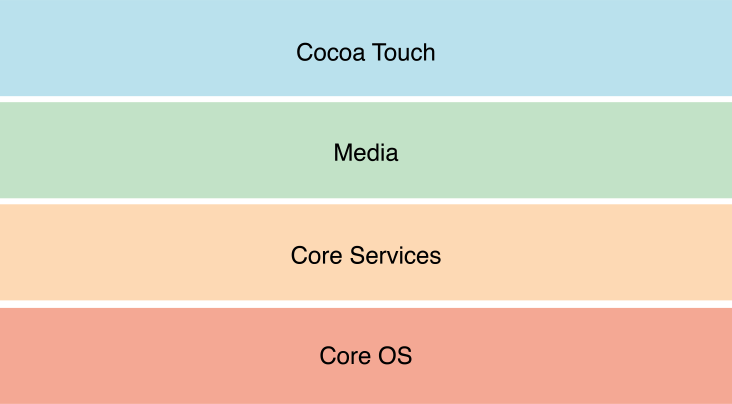
\includegraphics[scale=0.3]{figs_hwysw/iOSLayers.png}
\caption{Capas de iOS}
\label{fig: capas}
\end{figure}
%http://developer.apple.com/library/ios/#DOCUMENTATION/AudioVideo/Conceptual/AVFoundationPG/Articles/00_Introduction.html#//apple_ref/doc/uid/TP40010188
As� entonces, dentro de cada capa existen distintos \textit{Frameworks} seg�n la funcionalidad. A continuaci�n se explica un poco m�s en detalle el rol de cada capa, los distintos \textit{Frameworks} que tiene cada una y para qu� sirven.
\subsubsection{Cocoa Touch Layer}
Cocoa Touch es la capa de m�s alto nivel de iOS y es la encargada de proveer al desarrollador de ciertos \textit{Frameworks} que permitan lograr distintas tecnolog�as como la posibilidad de multitarea, el ingreso de �rdenes a la aplicaci�n a trav�s de la pantalla t�ctil, notificaciones y alertas, preservaci�n del estado de la aplicaci�n al salir de la misma, reconocimiento de gestos en la pantalla y otro tipo de funcionalidades de alto nivel. Permiten al desarrollador, sin tener que involucrarse demasiado a bajo nivel, el acceso a determinados servicios que ya est�n resueltos en forma bastante modular.\\
Cocoa Touch est� basado en la arquitectura \textbf{Modelo-Vista-Controlador}, en el que se separa en tres �reas distintas el modelo de la informaci�n, la interfaz de usuario y el conjunto de reglas que negocian la presentaci�n de la informaci�n en base a la interacci�n con el usuario. As� pues, el usuario y una aplicaci�n se podr�an considerar dos sistemas que interaccionan. Por su parte el usuario tiene como entrada la vista de la aplicaci�n y como salida tiene su respuesta a esta entrada, generando efectos sobre el control de la aplicaci�n. Por otro lado la aplicaci�n tiene como entrada las �rdenes dadas por el usuario que tienen efectos sobre el modelo de la informaci�n y este sobre la vista, quien resulta ser la salida de la aplicaci�n. Esta interacci�n se puede ilustrar con la figura \ref{fig: mvc}.
\begin{figure}[h!]
\centering
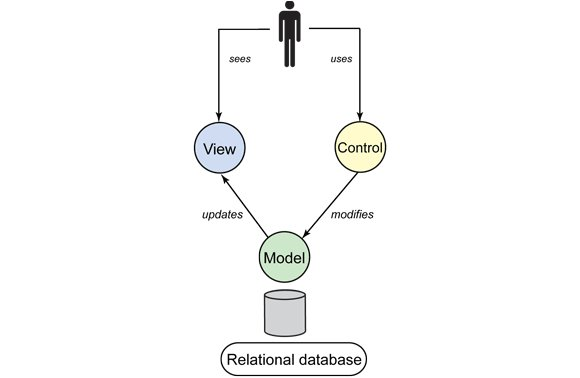
\includegraphics[scale=0.6]{figs_hwysw/mvc3.png}
\caption{Interacci�n entre las tres partes del MVC}
\label{fig: mvc}
\end{figure}
%http://developer.apple.com/library/mac/#documentation/Cocoa/Conceptual/ObjectiveC/Introduction/introObjectiveC.html 
Como se dijo, dentro de Cocoa Touch, existen distintos \textit{Framewokrs} enfocados en permitirle al desarrollador resolver en alto nivel distintos aspectos. Los mismos son los siguientes:
\begin{itemize}
\item[(1)] Address Book UI Framework
\item[(2)] Event Kit UI Framework
\item[(3)] Game Kit Framework
\item[(4)] iAd Framework
\item[(5)] Map Kit Framework
\item[(6)] Message UI Framework
\item[(7)] Twitter Framework
\item[(8)] UIKit Framework
\end{itemize}
Quiz� sea bueno mencionar que varias de estas API no fueron utilizadas en el presente proyecto dada su funci�n espec�fica y que no fueron necesarias. Sin embargo hay una en particular que tiene bastante importancia y que permite la mayor�a de las funcionalidades b�sicas que toda aplicaci�n tiene. Se trata del \textbf{UIKit}, encargado de gestionar la aplicaci�n, su interfaz de usuario y gr�ficos, encargado soportar eventos frente al toque de la pantalla, de manejar sensores como el aceler�metro y giroscopio, y de tener acceso a la c�mara y galer�a de fotos entre lo m�s importante a destacar. El soporte de la multitarea y de \textbf{Storyboards} tambi�n est� a cargo de este \textit{Framework}.\\
Hay funcionalidades que han ido cambiando con las distintas versiones de iOS. Una de ellas y quiz� una que ha generado bastantes diferencias respecto a versiones anteriores a iOS 5, es esta �ltima, el Storyboard, una herramienta muy �til de programaci�n gr�fica, que permite generar instancias de clases y v�nculos entre las mismas en forma visual a la vez de ser una contraparte de interfaz de usuario. Con una biblioteca de objetos disponibles, listos para ser usados, mediante el uso de Storyboard se hace accesible con algunas horas de dedicaci�n implementar aplicaciones sencillas. Esta herramienta vino para sustituir los archivos \textit{.nib} que permit�an dise?ar la interfaz pero no tantas funcionalidades program�ticas como el Storyboard. En particular �ste �ltimo permite agregar la funcionalidad de \textit{segues}, encargados de vincular un \textit{ViewController} con otro. Este tipo de diferencias vinieron con la idea de evitar la necesidad de implementar ciertos bloques de c�digo en forma repetitiva. Un Storyboard luce como en la figura \ref{fig: story}.
\begin{figure}[h!]
\centering
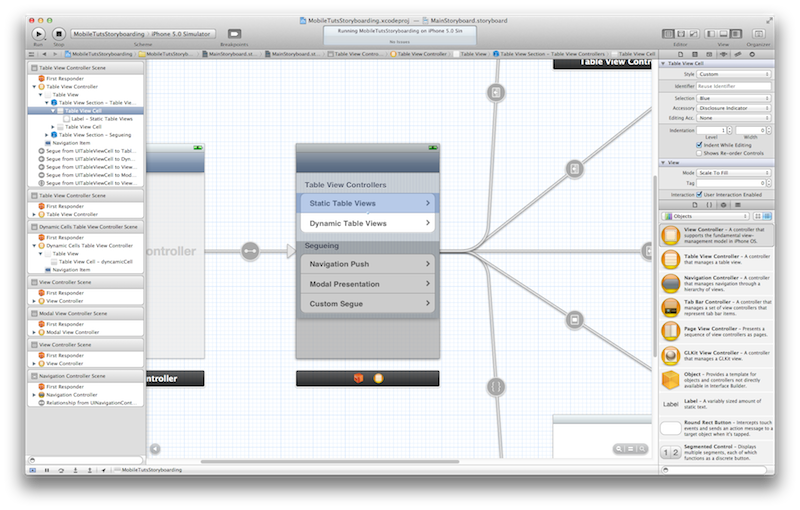
\includegraphics[scale=0.3]{figs_hwysw/story.png}
\caption{Ejemplo de Storyboard.}
\label{fig: story}
\end{figure}

Si bien se podr�a extender bastante m�s la explicaci�n sobre los detalles de Cocoa Touch, a los efectos del presente proyecto, no es de tanta relevancia excederse en este punto. 
\subsubsection{Media Layer}
\textit{Media Layer} es la capa encargada de gestionar correctamente elementos multimedia y es posible ditinguir tres grandes grupos que engloban distintos \textit{Frameworks}: Gr�ficos, Audio y Video. \\
Dentro de las tecnolog�as m�s destacadas est� todo lo vinculado a \textbf{gr�ficos} 2D y 3D, dentro de lo que se puede incluir algunos \textit{Frameworks} bastante utilizados en el presente proyecto, tales como: \textbf{Core Graphics}, muy utilizado para dibujos 2D, \textbf{Quartz Core}, quien contiene las herramientas necesarias para interactuar con otro \textit{Framework} para animaci�n de vistas, de una capa de m�s bajo nivel como \textit{Core Animation}, que es comentado m�s adelante en la secci�n \ref{sec: coreserv}. Tambi�n es parte de lo vinculado a gr�ficos, el \textit{Framework} \textbf{Core Image}, conteniendo lo vinculado a procesamiento de im�genes a trav�s filtros que utilizan directamente la lu unidad de procesamiento de gr�ficos (GPU) y otros dos \textit{Frameworks} bastante importantes en lo que respecta a \textit{rendering} como \textbf{Open GL ES} y \textbf{GLKit} (utilizado por el motor de juegos \textit{Isgl3d} entre otros).\\
Por otra parte hay otra gran familia de \textit{Frameworks} dentro de Media Layer que apunta a resolver todo lo vinculado al manejo de audio, ya sea de grabaci�n como procesamiento y reproducci�n de alta calidad. Existen algunos SDK como \textbf{iSpeech} o \textbf{Dragon Mobile} que resuelven de manera similar al proyecto Siri, el procesamiento de la voz humana reconociendo palabras e interpretando, que utilizan algunos de los \textit{Frameworks} de procesamiento de audio de esta familia. \\
En cuanto a lo vinculado al manejo de video, como parte de esta capa, se tienen dos \textit{Framework} importantes con distintos niveles de abstracci�n: \textbf{MediaPlayer} y \textbf{AVFoundation}. Tambi�n existen otros \textit{Frameworks} fuera de esta capa que son capaces de manejar video como la clase UIImagePickerController (muy utilizada en el proyecto) del mencionado UIKit. En la figura \ref{fig: avfound} se esquematiza el nivel de abstracci�n de los \textit{Frameworks} de las distintas capas que son capaces de manejar multimedia.
\begin{figure}[h!]
\centering
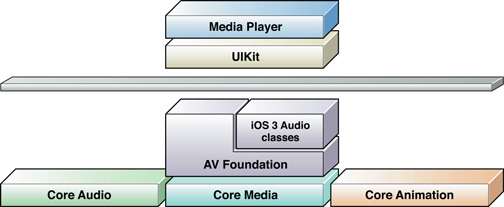
\includegraphics[scale=0.6]{figs_hwysw/avFoundation.png}
\caption{Frameworks de las distintas capas para manejo de video}
\label{fig: avfound}
\end{figure}
Con MediaPlayer es posible reproducir audio y video muy f�cilmente en determinada �rea de la pantalla ya sea desde un URL o de un archivo, es posible mostrar o no los elementos de control del video as� como tambi�n controlar, volumen y tama?o de la pantalla. Por su parte, con AVFoundation es posible capturar con la c�mara, reproducir, editar y procesar audio y video. Es posible implementar ciertos protocolos que hace de esto algo relativamente sencillo. 


\subsubsection{Core Services}
\label{sec: coreserv}
Core Services es la capa de m�s bajo nivel de iOS y contiene los elementos fundamentales sobre los que se construyen las capas superiores. Es posible que al comenzar a programar para iOS no se tenga mucha interacci�n con esta capa pero sin embargo existen algunos conceptos importantes de esta capa que s� vale la pena mencionar dado que en el presente proyecto se tuvieron que entender y discutir. Una de ellas es la \textit{Automatic Reference Counting} o \textbf{ARC}. Esta funcionalidad compete a la reserva y liberaci�n de memoria por parte de los objetos. La idea b�sica es lograr que el uso de memoria sea el m�nimo posible, logrando que los objetos existan en la medida que son necesarios y que su memoria sea liberada ni bien sea posible. 
\begin{figure}[h!]
\centering
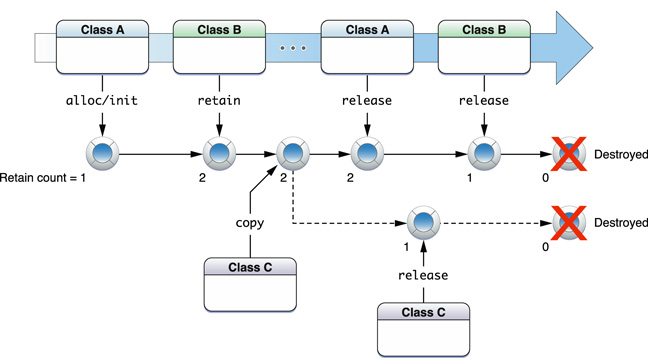
\includegraphics[scale=0.6]{figs_hwysw/mrr.png}
\caption{Ciclo de vida de objetos, Manual-Retain-Release.}
\label{fig: manualRR}
\end{figure}
T�picamente, al crear una instancia de un objeto se incrementa un contador y al liberar se decrementa y entonces se tiene cierto control sobre la reserva y liberaci�n de memoria en base al contador. Sin embargo, la liberaci�n de memoria reservada por objetos queda bajo la responsabilidad del desarrollador y en casos de un c�digo complejo puede llegar a ser habitual olvidarse de la liberaci�n de memoria.	 Lo anterior refiere a una gesti�n manual de la reserva y liberaci�n conocido como \textit{manual retain-release}. Para no tener que enfrentar este tema y poder instanciar clases sin tener presente la posterior liberaci�n de memoria (pues quiz� se sepa cu�ndo no ser� m�s necesario un objeto o no), se utiliza ARC. Esta funcionalidad eval�a el ciclo de vida de los objetos y agrega c�digo en tiempo de compilaci�n en caso de considerarlo necesario. Es bueno aclarar que esto refiere a memoria reservada pura y exclusivamente por objetos, es decir mediante \textit{alloc}. En caso de tratarse de memoria reservada para variables de lenguaje C (\textit{malloc}), es necesario proceder de igual manera que en dicho lenguaje, liberando la memoria mediante un \textit{free}. \\
Adem�s del ARC, Core Services permite el manejo de archivos XML y manejo de base de datos SQL as� como tambi�n la protecci�n de datos cuando el dispositivo est� bloqueado entre otros servicios importantes. Tiene varios \textit{Frameworks} como \textbf{Core Media} que logran un nivel a�n m�s bajo que AVFoundation para el manejo de multimedia, \textbf{Quick Look} para las vistas previas de archivos, \textbf{Social} que viene a suplantar el \textit{Framework} para la utilizaci�n de Twitter que existe en iOS 5 y extiende la gesti�n para otras redes sociales, \textbf{Core Motion} para el manejo de sensores como el aceler�metro y el giroscopio, \textbf{Core Telephony} para el manejo de la informaci�n de red del dispositivo como elemento de la red de telefon�a, \textbf{CFNetwork} para el manejo de protocolos de red como http, https, ftp y resoluci�n de servidores DNS, entre otros \textit{Frameworks} importantes dentro de la capa.
%manual reference counting http://developer.apple.com/library/ios/#documentation/Cocoa/Conceptual/MemoryMgmt/Articles/MemoryMgmt.html#//apple_ref/doc/uid/10000011i
% ARC http://developer.apple.com/library/ios/#releasenotes/ObjectiveC/RN-TransitioningToARC/Introduction/Introduction.html#//apple_ref/doc/uid/TP40011226
\subsubsection{Core OS}
Con esta capa de iOS en general es dif�cil que el desarrollador tenga que involucrarse directamente dado que es la de m�s bajo nivel. Salvo que se est� frente a una aplicaci�n que requiera aspectos de seguridad o comunicaci�n con HW externo, esta capa solamente existe para ser la base sobre la cual se desarrollan los \textit{Frameworks} de las capas de m�s alto nivel. Los distintos \textit{Frameworks} que tiene est�n enfocados en resolver temas de procesamiento basados en el hardware de iOS, en comunicarse con dispositivos externos basados en iOS y de garantizar la seguridad de los datos de una aplicaci�n.


\subsubsection{Simulador}
Uno de los detalles m�s importantes del entorno de desarrollo es la capacidad de simular lo que se programa antes de probarlo en un dispositivo. Esto es �til por cuestiones de seguridad e incluso permite programar sin la necesidad de contar con una plataforma. Esto existe para \textit{Xcode} y es necesario decir que funciona muy bien, generando una representaci�n bastante fiel de lo que sucede en el dispositivo real. La �nica cr�tica que se le podr�a hacer es el hecho de no contar con c�mara y para el caso de aplicaciones de realidad aumentada esto es algo bastante importante. Sin embargo, sin ser eso, el simulador cuenta con conexi�n a internet, pantalla multit�ctil, con informaci�n de GPS ingresada por el programador, acceso a la galer�a de fotos, capacidad de procesamiento y todas las funcionalidades que un dispositivo real tiene. 
\subsubsection{Instruments}
%https://developer.apple.com/library/ios/#documentation/DeveloperTools/Conceptual/InstrumentsUserGuide/Introduction/Introduction.html#//apple_ref/doc/uid/TP40004652
Dentro de las herramientas que vienen con el entorno de desarrollo viene \textit{Instruments}, un conjunto de herramientas que permiten analizar la performance de una aplicaci�n para iOS o para Mac OS X desde distintos puntos de vista. Resulta muy �til pues muchas veces sucede que una aplicaci�n compila y se ejecuta correctamente y sin embargo puede que el desarrollador no est� conforme en cuanto a los tiempos de procesamiento o el uso de memoria consumido.\\
Para poder hacer uso del \textit{Instruments}, es necesario correr la aplicaci�n en modo \textit{Profile}. Eso despliega una ventana como la de la Figura \ref{fig: instru}. All� es posible elegir dentro de cada una de las posibilidades que ofrece \textit{Instruments}, si se quiere analizar tiempos, memoria, recursos de CPU, \textit{multithreading} entre otros tipos de datos de inter�s que es posible recoger de la aplicaci�n. Tambi�n es posible elegir la plataforma, ya sea iOS, simulador iOS o Mac OS X.\\

\begin{figure}[h!]
\centering
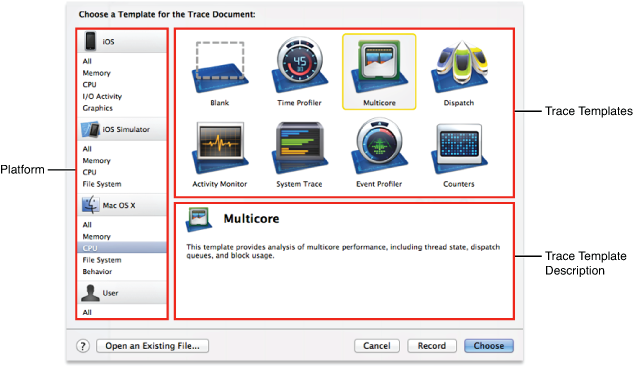
\includegraphics[scale=0.6]{figs_hwysw/instrumentsWindow.png}
\caption{Distintas opciones de \textit{Instruments}.}
\label{fig: instru}
\end{figure}
Luego de elegir el tipo de datos a ser recolectados seg�n lo que se busque analizar, se despliega una ventana como se ve en la Figura \ref{fig: instru2}. All� es necesario registrar durante varios segundos los datos mientras se corre la aplicaci�n y luego de terminado el registro, \textit{Instruments} dedica un tiempo a analizar los datos recolectados. En el detalle inferior, se desglozan los procesos que corre la aplicaci�n en forma de �rbol. Cuando se desea medir tiempos por ejemplo, esto resulta muy �til porque entre otras cosas se puede analizar qu� porcentaje del tiempo de la aplicaci�n es consumido por un m�todo en particular. Esto es posible simplemente buscando dentro del �rbol mencionado, al m�todo y leyendo el valor asignado de tiempo. Para el caso de an�lisis de memoria tambi�n es posible identificar f�cilmente en qu� parte del c�digo se est� dando alg�n problema de reserva de memoria no liberada.
\begin{figure}[h!]
\centering
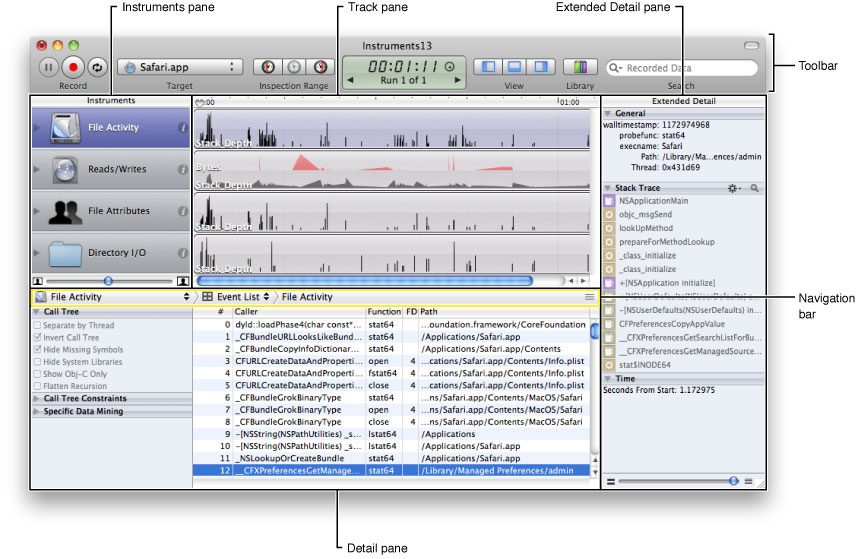
\includegraphics[scale=0.6]{figs_hwysw/instruments_tracing.png}
\caption{Trazado y an�lisis de datos recogidos.}
\label{fig: instru2}
\end{figure}
En el presente proyecto se hizo uso principalmente del \textbf{Time Profiler} que permite analizar tiempos y del \textbf{Memory Leak} que permite hacer un an�lisis de la reserva de memoria no liberada. Con los mismos fue posible optimizar tiempos en determinados m�todos del procesamiento, as� como tambi�n eliminar problemas de memoria no liberada que desencadenaban en la interrupci�n abrupta de la aplicaci�n luego de llegado un cierto nivel de reserva. Esta interrupci�n abrupta es una forma de proteger la memoria del dispositivo y evitar que se vea afectada cierta memoria �til a otros efectos. El resto de las herramientas de \textit{Instruments} fueron probadas pero no utilizadas en detalle para resolver problemas particulares.

\section{Herramientas}
Herramientas
\subsection{GIT}
\subsection{GoogleCode}
\subsection{Github}



% Ejemplo de como hacer una cita:
%\cite{Daniel03simultaneouspose}.



\bibliographystyle{unsrt}   
\bibliography{encuadro}  
\end{document}
